\section{Arkitektur}\label{sec:arkitektur}
Dette afsnit præsenterer arkitekturen som er udarbejdet på baggrund af de specificerede behov i \cref{arkitekturkrav}.

\paragraph{Platform}
Projektet har valgt at bruge Android platformen, se \cref{sec:valg_af_android}, som også lægger op til nogle overvejelser ift. arkitektur.

Arkitekturen er lavet ud fra ideen om at applikationer på Android kan kontakte hinanden igennem Android systemet.
Det er muligt for en hovedapplikation at starte en service der ligger i en anden applikation \cite{android_service}.
Dette udnyttes ved at pakke alle moduler i hver deres selvstændige applikation.
Ved at anvende en centraliseret database vil det være muligt for moduler at få adgang til data fra andre moduler.
Samtidig kan adgangsrettigheder til de forskellige tabeller styres et sted.
På den måde kan adgang kontrolleres på alle moduler, inklusiv de der måtte blive udviklet i fremtiden.
Hertil ønskes en central styrende enhed, der skal fungere som bindeled mellem de installerede moduler.

\section{Opbygning}\label{arkitektur:opbygning}
Den overordnede arkitektur er opbygget af fire komponenter: \textit{manager}, \textit{moduler}, \textit{DB\footnote{Database} access} og \textit{DB}.
For at opfylde de specificerede behov i \cref{arkitekturkrav}, nærmere nøgleordene \textit{modulær}(se \cref{arkitekturkrav::modulaer}) og \textit{fleksibel}(se \cref{arkitekturkrav::fleksibel}) er arkitekturen opbygget af moduler der opsamler data, analyser denne data og viser den uafhængige af hinanden.
Disse moduler kan vælges til eller fra i \textit{manager}'en.


Et diagram over arkitekturen kan ses på \cref{arkitektur_udkast_1}.
\begin{figure}[h]
	\centering						%  l   b   r	t
	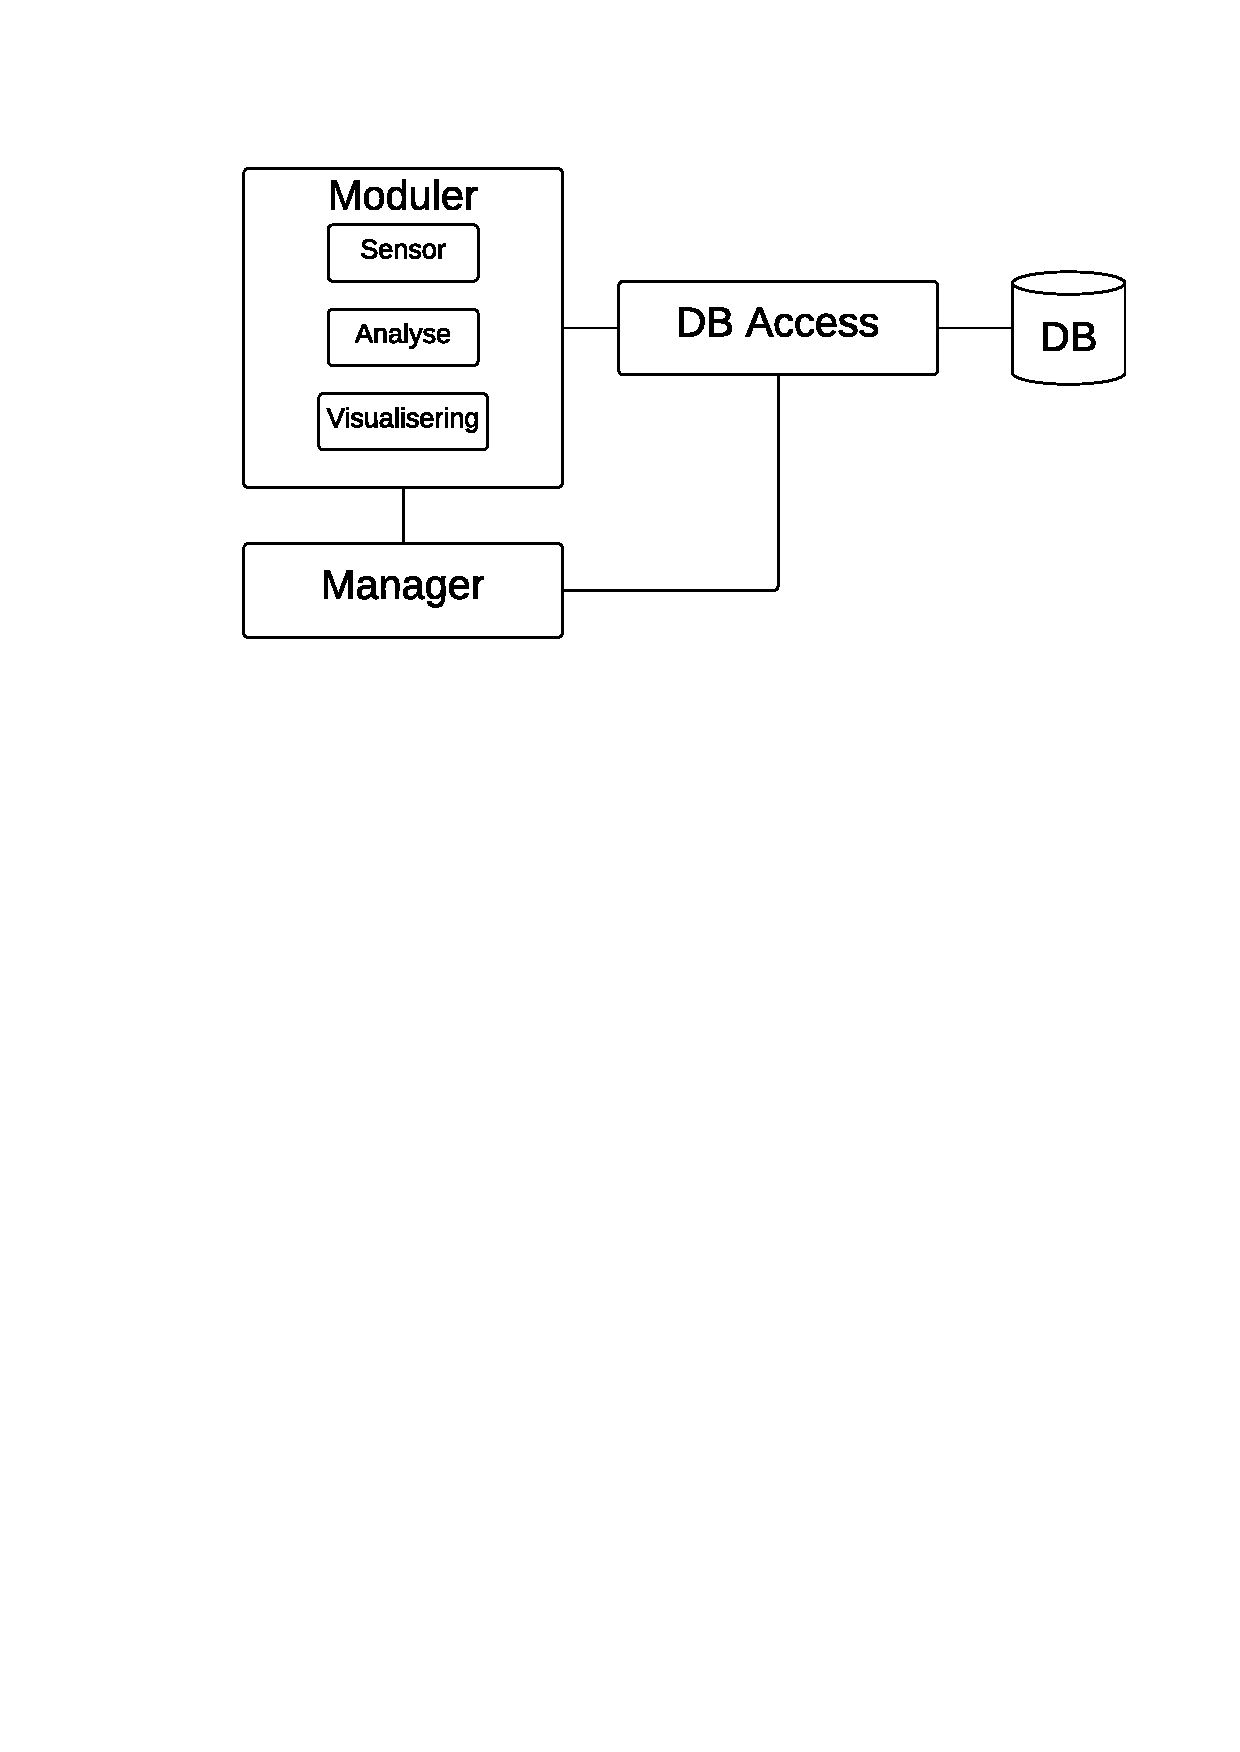
\includegraphics[scale=0.5, trim = 1cm 17.5cm 1cm 1cm, clip]{ArkitekturLucidChart}
	\caption{Systemets arkitektur}
  \label{arkitektur_udkast_1}
\end{figure}

Herunder gives en beskrivelse af hver af de fire komponenter.
Komponenterne beskrives i rækkefølge af deres indbyrdes afhængighed, således at forståelsen af hver komponent kun afhænger af det læste.

\subsection{DB}
Denne komponent administrerer data for systemets forskellige moduler.
Data opbevares i en række tabeller i et relationelt database system.
Hvert modul har mulighed for at definere egne tabeller, der alle gemmes i \textit{DB} komponenten.

Til dette projekt er valgt en SQLite database da denne er standard i Android \cite{android_database}.


\subsection{DBAccess}\label{subsec:DBACCESS}
Denne komponent styrer adgangen til \textit{DB} komponenten så det sker på en ensrettet måde.
Da vi arbejder på en mobil platform er det værd at tage højde for lagerstyring og abstraktion derover.
Da der er begrænset plads på en smartphone kan det blive relevant at lagre noget af det indsamlede data i skyen.
Grundet denne potentielle opdeling af lager placeringer, kan de være nyttigt at abstrahere over hvor data lagres.

For at opfylde nøglepunktet \textit{kommunikation}, se \cref{arkitekturkrav::kommunikation}, er det nødvendigt at sørge for at moduler har adgang til kun at skrive til deres egen database og samtidig læse fra alle andres database.
På denne måde forhindres det at eksterne moduler modificerer andre modulers data.

\paragraph{Design} 
For at imødekomme kravene om både at give ensrettet adgang til moduler og stille garantier om adgangsrettigheder er der blevet valgt at benytte facade designmønster \citep[s.~185]{gamma1994design}.

Grunden til at facade er benyttet er fordi det giver en kobling mellem moduler og databasen.
Denne kobling sker gennem et interface der sørger for modulerne kun skal opfylde nogle få krav for at få deres data gemt i databasen, samt for at få data fra andre moduler.
Endvidere, sørger den kobling for at skabe en specifik og sikker kommunikation mellem moduler sker nemt og sikkert, hvilket er nødvendigt for at opfylde nøglepunktet \textit{kommunikation}, se \cref{arkitekturkrav::kommunikation}.

\subsection{Moduler}
Denne komponent befinder sig i et lag for sig selv og indeholder tre typer moduler: \textit{data}, \textit{analyse} og \textit{visualisering}.
Komponenten indeholder applikationens hovedfunktionalitet og er ansvarlig for indsamling af data, bearbejdelse af data og visualisering af data.

Dette afsnit beskriver hvordan modulerne er defineret og en beskrivelse af de tre typer moduler.
Men først en begrundelse for valget af dette lag på baggrund af behovene i \cref{arkitekturkrav}.

\paragraph{Begrundelse for valg}
For at opfylde nøgleordet \textit{modulær}(se \cref{arkitekturkrav::modulaer}) er det valgt lave et lag der indeholder moduler, så det er let at tilføje og fjerne moduler.
Dette kunne fx være i en situation hvor der kommer nye sensorer på markedet, eller hvis der skal laves nye former for visualiseringer til det allerede indsamlede data.

\subsubsection{Moduldefinition}\label{modul_definition}
%Måde at lave eksterne modul-applikationer uden at ændre hoved-applikation.
%Definere output (tabeller/kolonner), samt input (afhængigheder)
%Evt. konfigurationsmuligheder for moduler afhængige af det
%Fleksibel måde at modtage data fra andre moduler, uden at skulle opdatere applikation(erne). Dvs. ikke design-mønstre: observer, mediator, men gennem content provider.
% modularisering i Android; multiple applikationer under samme package

For at opfylde kravet om fleksibilitet der er stillet til systemet, har vi udtænkt en modulbaseret arkitektur der gør det let at tilføje moduler til pakken.
Det skal være muligt at tilføje eksterne moduler, uden at have behov for at lave ændringer i hoved-applikationen.
Dette kan gøre sig gældende når der kommer nye sensorer på markedet, eller hvis der skal laves nye former for visualiseringer til det allerede indsamlede data.
\subsubsection{Forslag til modulariseing}
\paragraph{Komplet Pakke}
En traditionel applikation samler al funktionalitet i en pakke.
Hvis man udvikler på dele af applikationen vil en opdatering skulle ske af hele appen på samme tid.
Desuden bliver det sværere for eksterne udviklere at bidrage til applikationen, da opdateringer skal ske igennem udviklerne af hovedapplikationen.

\paragraph{Import af Kode}
En anden mulighed er at inkludere et scripting sprog med applikationen og gøre det muligt at udvikle script der kan agere modul.
Denne løsning kræver et meget kraftigt scripting sprog hvis alle Androids muligheder skal stilles til rådighed.
Hvis scripts på den anden side skal skrives direkte i java vil der være nogle sikkerhedshensyn som vil gøre det svært at kontrollere hvad moduler kan og ikke kan.
For eksempel vil det være vanskeligt at kontrollere hvilke database tabeller der er adgang til.
Sikkerhedsproblemet er stort, men kunne sikkert løses med nok tid og ressourcer.

\paragraph{Selvstændig Applikation}
Den tredje mulighed er at pakke hvert modul i en selvstændig APK \footnote{Androids pakkeformat}.
Denne APK skal indeholde en beskrivelsesfil som læses i hoved-applikationen og indeholder information om modulet.
Denne metode sørger for at hoved applikationen kan kontrollere hvad moduler har adgang til. 

Ulemper ved denne løsning er at den er knap så lightweight, idét at det kræver at en stor mængde af applikationer skal installeres.
Derudover er kommunikation mellem applikationer vanskeligere end internt i en applikation, men ses som acceptabelt.
Desuden kan det være træls at skulle installere en større mængde af applikationer for at have den fornødne funktionalitet.
Som løsning derpå kunne man med videre arbejde have et indbygget applikation marked i manageren, og er værd at udforske med mere tid.

Det er en løsning der har mange fordele i forhold til modularisering og svagheder der kan tolereres, hvorfor denne løsning er valgt. 

Det følgende vil forklare detaljerne i implementationen af moduler ved hjælp af selvstændige applikationer.

\subsubsection{Beskrivelsesfilen}

Til dette er der valgt at bruge JavaScript Object Notation (JSON) samt JSON Skema \citep{jsonpojo}.
Eksemplerne der bruges herefter vil derfor være i henholdsvis JSON eller JSON Skema.

\subsubsection{Typer af Moduler}
Der findes som sagt i \cref{sec:arkitektur}, tre typer moduler: \textit{sensor}, \textit{analyse} og \textit{visualisering}.
Som sagt er sensor moduler, moduler som indsamler data fra telefonens forskellige sensorer og applikationer.
Endvidere er analyse moduler, moduler som bruger data fra enten sensor eller andre analyse moduler til at bearbejde data med den hensigt at opnå en opsummering af data som kan videre bruges af systemet til enten visualisering eller videre bearbejdning.
Visualiseringsmodulerne bruges til visualisering af den rå sensor-data eller den behandlede analyse-data.

\subsubsection{Moduldefinition}
Som minimum har et modul et navn og en version, så andre moduler kan referere dem.

Sensor- og analyse-moduler skal gøre data tilgængeligt for andre analyse- og visualiserings-moduler.
For at specificere hvordan data skal gemmes, samt hvad der er tilgængeligt for andre, skal dette defineres for hvert modul af førstnævnte typer.
For hvert modul skal der defineres en eller flere tabeller som modulet kan gemme data i.
For hver tabel defineres en eller flere kolonner med et beskrivende navn, datatype og evt. en måleenhed.

\subsubsection{Data Typer}
De tilgængelige data typer tilgængelig for tabel-kolonner, er begrænset til de tilgængelige SQLite datatyper.
Der er 5 typer: \textit{NULL}, \textit{INTEGER}, \textit{REAL}, \textit{TEXT} og \textit{BLOB}.

\subsubsection{Afhængigheder}
Et analyse- eller visualiserings-modul kan være afhængigt af andre sensor- eller visualiserings-moduler.
Et analysemodul kan aggregere data fra andre analysemoduler mens et visualiseringsmodul er afhængig af det modul det skal vise data fra.
Derfor skal det defineres for hvert modul hvilke andre moduler det er afhængigt af.
Der findes to grader af afhængigheder i systemet: hard- eller soft-dependency.
En hard-dependency er ét andet modul som det pågældende modul ikke kan fungere uden.
En soft-dependency er en liste af andre moduler, hvor mindst ét af de listede moduler skal være til stede på enheden.
Dette er nyttigt hvis et modul skal bruge eksempelvis accelerometer data, men det er ikke vigtigt om det kommer fra en telefon eller fra en wearable.

\subsubsection{JSON og JSON Schema}
For at have en modul-beskrivelse der er læselig for både mennesker og maskiner, er JSON valgt.
JSON gør det muligt for ikke-tekniske personer at læse, skrive og forstå definitionen af et modul.
For at sikre validiteten af eksternt leverede modul-beskrivelser, udarbejdes der et JSON Skema, som JSON-dokumenter kan holdes op imod og derved verificeres.
Det anvendte JSON Skema kan findes i \cref{app:json_schema}.

\paragraph{Eksempel} på en modul-beskrivelse.
Meta-data er præfikset med \_ (underscore).
\begin{lstlisting}
{
  "name": "accelerometer",
  "_version": 1.0,
  "tables": [
    { "name": "accelerations",
      "columns": [
        { "name": "accX",
          "dataType": "REAL",
          "_unit": "g" },
        { "name": "accY",
          "dataType": "REAL",
          "_unit": "g" },
        { "name": "accZ",
          "dataType": "REAL",
          "_unit": "g" }
      ]}]}
\end{lstlisting}

\subsubsection{Implementering}
Som nævnt i \cref{sec:valg_af_android}, implementeres der til Android telefoner.
Dette sætter nogle begrænsninger ift. valg af løsninger.

\subsubsection{JSON kontra XML}
XML ville være det naturlige valg for Android applikationer, da en del af applikations udvikling foregår i XML fordi man ofte bruger det til at definere layouts og definering af statiske ressourcer. 
Dog blev JSON valgt over XML, da vi gerne ville have automatisk generering af en parser ud fra skemaet.
En automatisk genereret parser vil lette arbejdet med et skema der i udviklingsperioden ændres ofte.
Denne automatiske generering viste sig ikke at være ligetil på grund af kompatibilitetsproblemer på Android, mens det var enkelt at udføre i JSON.

\subsubsection{Moduler som Applikationer}
For at det skal være muligt at installere moduler uden at opdatere hoved-applikationen, skal der installeres applikationer via Google Play Store.
Alle modul-applikationer, samt hoved-applikationen, deler \textit{package}-navn.
Hver modul-applikation har sin JSON beskrivelse som en eksternt tilgængelig \textit{ressource}, som hoved-applikationen eller andre moduler har adgang til.
Kommunikation mellem applikationer foregår med \textit{services}, \textit{intents} eller \textit{content provider}.

\subsubsection{Håndtering i Manager}
Håndteringen af moduler sker i manageren, beskrevet i \cref{subsec:arkitektur-Manager}.
Når der tilføjes eller opdateres et modul detekterer manageren dette ved at finde alle applikationer der er installeret under pakken ``dk.aau.cs.psylog''.
Manageren læser alle moduldefinitioner efter at have valideret dem op imod JSON skemaet.
Alle moduler der har opdateret versionsnummer eller er helt nye vil blive håndteret ved at manageren læser tabelinformation ind fra moduldefinitionen og opretter eller ændrer de pågældende tabeller.

Når modulernes tabeller er blevet oprettet bygges en graf over afhængigheder, som bruges til at vise brugeren hvilke moduler der kan aktiveres.
Denne proces er yderligere beskrevet i \cref{sec:settings}

\subsubsection{Visualiserings Modul}\label{sec:visningsmodul}
Som udgangspunkt er \textit{visualiseringer} forskellige visualiseringer af analyse modulernes output.

De eneste restriktioner der stilles for data der kan læses fra et analyse moduler er de formater der kan gemmes i databasen.
Det betyder at det mulige output fra et analyse model er meget fleksibelt, hvilket kræver en tilsvarende fleksibilitet i visualiseringsmodulerne.

En simpel løsning vil være at der for hvert analysemodul skal defineres et visualiserings modul.
Herved sikres det at alle analysemoduler har en visualisering der præcist repræsenterer genererede data.
Det er dog nemt at finde problemstillingerne i denne løsningsmodel, da det giver meget lav genanvendelse af eksisterende moduler.
Eksempelvis kan man nemt forestille sig forskellige datasæt der kan repræsenteres ved hjælp af en to-dimensional graf.
En løsning der ville kræve en ny implementation af en sådan visualisering for hver analyse modul er ikke fleksibel nok.

Alternativt kan visualiseringer beskrive en liste over de analyser de kan anvendes på.
På den måde kan visualiseringer anvendes på mere end et analyse modul.
Omend dette løser problemet til en vis grad vil problemet stadig eksistere når der tilføjes nye analyse moduler.
Her vil visualiseringerne enten ikke have kendskab til de nye moduler eller de vil skulle opdateres løbende.
Altså er fleksibiliteten af denne løsning heller ikke god nok.
Man kan naturligvis også lade alle analyse moduler beskrive en liste over visualiserings moduler.
Men denne opbygning vil give samme problemstilling som beskrevet herover.

En mere fleksibel metode til håndtering knytningen mellem visualiseringer og analyser er at deducere ud fra analysens tabel/kolonne signatur, hvilke slags data der kan aflæses.
På denne måde kan der laves visualiseringer der repræsenterer bestemte signaturer, og der opstår en implicit binding mellem visualiseringer og analyser for de hvor de to beskrivelser stemmer overens.

I mange tilfælde vil denne implicitte binding være nok, dog kan det forestilles at analyserne vil være forskellige og til tider komplekse, hvilket kan gøre det nødvendigt at nærmere specificere hvordan den tilgængelige data kan vises.
Der er også den mulighed at analysemoduler kunne have ekstra database tabeller, der ikke skal vises, som så kunne virke forstyrrende for den implicite binding.
Her kunne der tilføjes noget meta-data på analysens tabeller/kolonner, der beskriver den på sådan en måde, at det ville kunne bruges til visualiseringer der ikke nødvendigvis implicit kunne knyttes til det.
Det kunne også være muligt at tilføje information om kriterier for visualiseringer i analysemodulers JSON filer, og så overlade det til Manager komponenten at matche et analysemoduls kriterier med de kriterier visningsmoduler opfylder.

\subsubsection{Eksempel}
Her bruges light, som er en simpel sensor og analyse, der fra sensoren indhentes løbende lys-niveau (i lux).
Analysen tager den senest indsamlet data og giver et gennemsnit.
Det antages at alle tabeller har en tids-kolonne, der beskriver enten hvornår data blev indsat i databasen, eller i nogle tilfælde af analyser overføres tiden fra sensor-data.

\begin{lstlisting}
{
  "name": "lightAvg",
  "_version": 1.0,
  "tables": [
    {
      "name": "lightAvg",
      "columns":[
        { "name": "lightAvg", "dataType": "REAL", "_unit": "lux" }
      ]
    }
  ],
  "dependencies": [
    [{ "name": "light" }]
  ]
}
\end{lstlisting}

Et eksempel på et visualiserings-modul som passer på denne type analyse kunne være en simpel 2D graf, som viser den gennemsnitlige belysning over tid.

\begin{lstlisting}
{
  "name": "2dgraph",
  "_version": 1.0,
  "_type": "view",
  "view": {
    "layout": "2dgraph.xml",
    "data": [
      { "name": "x", "dataTypes": ["INTEGER"], "fromTimestamp": true },
      { "name": "y", "dataTypes": ["INTEGER", "REAL"] }
    ]
  }
}
\end{lstlisting}
 
Denne visualisering beskriver en 2D graf, som bruger layoutet i \texttt{2dgraph.xml}.
På x-aksen vises tiden (der står INTEGER fordi SQLite ikke har datorepræsentation ud over unix-time).
Her bruges det tidsstempel som forventes på alle tabeller.
Til y-aksen kan bruges alle analyser, som blot har en enkelt kolonne af heltal eller decimal-tal værdi.

\subsubsection{Administrering af Visualiseringer}
Ligesom sensorer og analyser, skal visualiseringer også administreres af brugeren.

For at holde det så simpelt som muligt, kunne man, ligesom ved sensorer/analyser, have to niveauer af administration.
Som udgangspunkt vil alle installerede visualiseringer automatisk knytte sig til de aktiverede analyser.
Derudover vil man i de avancerede indstillinger kunne aktivere/deaktivere visualiseringer for de enkelte analyser.

På denne måde vil der automatisk blive genereret en liste af visualisering/analyse kombinationer, men med mulighed for at slå nogle af kombinationerne fra.
Det vurderes at muligheden for at slå visualiseringer fra skal være under avancerede indstillinger, da ikke teknisk erfarne brugere sagtens kunne forvirres af alle de potentielle visualisering/analyse kombinationer de ville præsenteret for.
Grunden til at det stadig er med som en mulig customization er, at der er stor fokus på at brugerne skal have mulighed for at styre hvad programmet skal gøre. 


\subparagraph{Data}
\textit{Data}-laget indeholder moduler der indsamler data fra smartphonens (eller tilbehør dertil) forskellige sensorer og applikationer.
Der påføres kun et minimum af behandling på indsamlede data (eksempelvis komprimering) således at data kan indsamles kontinuert uden stort energi-behov.
Derudover for at have mulighed for at lave meningsfulde analyser skal alt logget data gemmes i \textit{DB} i rå eller komprimeret form.
Det vil sige at komprimering skal være tabsfri og at eventuelle fejlmålinger bør markeres som sådan i den pågældende data tabel.

Et eksempel på et sensormodul er indsamling af data fra accelerometret.
Modulet får data fra accelerometret og gemmer det i sin database. 
For ikke at gemme unødvendige mængder data vil modulet kun gemme et datapunkt når det er forskelligt fra det forrige målte punkt.

\subparagraph{Analyse}
\textit{Analyse}laget indeholder moduler der bruger data fra et antal sensormoduler samt eventuelle andre analysemoduler.
Herefter udføres en analyse af det indsamlede data med \textit{''forståelig information''} som resultat.
I denne process vil der kunne forekomme tab af data.
Herved opnås en opsummering af det indsamlede data, der skaber værdifuld information for brugeren.
Som en del af et analysemoduls beskrivelse findes en beskrivelse af hvilken information man kan få fra modulet.
Denne information anvendes af visualiseringsmodulerne.

Der kan ved analyse af sensordata anvendes flere ressourcer, da analysen typisk vil kunne udføres på større mængder indsamlede data få gange dagligt.
Eksempelvis kan analysen foretages om natten hvor smartphonen kan sættes til opladning.

Et eksempel på et analysemodul kan være et søvnanalyse modul der bruger førnævnte accelerometer data til at undersøge en sovendes søvn.
Dette modul vil bruge flere sensormoduler til sin analyse og vil muligvis bruge accelerometerdata fra både en smartphone og et smart watch.

\subparagraph{Visualisering}
\textit{Visualiserings}laget indeholder moduler der visualiserer analyserede data.
Som en del af et visualiseringsmoduls beskrivelse findes en beskrivelse af hvilken information modulet accepterer.
Hvis denne beskrivelse stemmer overens med et analysemodul, kan den enkelte visualisering anvendes på den enkelte analyse.

Et eksempel på et visualiseringsmodul er et modul der visualisere de resultater som føromtalte søvnanalyse har fundet frem til.
Dette kunne være en graf der fortæller hvor dyb søvn man har været i, eller en simpel farvet indikator hvis farve viser hvor godt man har sovet de sidste par dage.

Eksempelvis vil et accelerometer \textit{sensor}modul kunne anvendes af et søvn \textit{analyse}modul der viser resultatet i et graf \textit{visualiserings}modul.

Skulle man her ønske en anden fortolkning af accelerometerets data kan et andet analysemodul anvendes.
Sammensætningen af analyse- og visualiseringsmoduler sker ved en beskrivelse af deres grænseflade.
Moduler med fælles grænseflade vil kunne kombineres.
Det vil sige at der kan anvendes flere forskellige visualiseringsmoduler til det samme analysemodul, givet at de er kompatible.
Tilsvarende kan det samme visualiseringsmoduler anvendes til flere forskellige analysemoduler.

\subsection{Manager}\label{subsec:arkitektur-Manager}
Manager komponenten kan siges at være grænsefladen mellem bruger og moduler.
Den står for at administrere de installerede moduler ud fra de beskrivelser der er givet for de enkelte moduler.
Denne administration indebærer blandt andet oprettelse af de database tabeller hvert modul har bedt om i sin beskrivelse, samt start og stop af sensor- og analysemoduler.
Sidstnævnte sker ud fra definitioner givet i beskrivelserne af de enkelte moduler.
Desuden er det også gennem manageren brugeren for vist den information de leder efter.

\paragraph{Design}
Ved at sammenholde visualiseringer og analyser kan manageren beskrive for brugeren hvilke data der kan fremvises og med hvilke visualiseringer det kan ske.
Manageren har desuden en prædefineret brugerflade der anvender ovenstående kombinationer til at vise brugeren de relevante informationer.

Manager komponenten indeholder desuden et JSON skema for hver modul-type i moduler komponenten.
Disse definitioner beskriver formatet for eventuelle nye moduler man måtte ønske at føje til systemet.
\stefan{et eller flere skemaer? Muligvis har views anderledes skema, men analyse og sensorer har det samme}

